\documentclass[tikz,border=10pt]{standalone} 
\usepackage{tikz}
\usetikzlibrary{chains}
\usepackage[utf8]{inputenc}
\usepackage[T1]{fontenc}
\usepackage{lmodern}
\usepackage{varwidth}

\begin{document}

\tikzstyle{arrow} = [thick,->,>=stealth, line width=1.5pt, font=\sffamily]

%mdma = "[CH3][C][b2][HN][CH3][C][C1][C2][C3][C4][b3][O1][C][O2][r5][C5][C6][r6]" 

\begin{tikzpicture}

\begin{scope}[start chain=1, 
    every node/.style={on chain},
    bloc/.style={fill=red!80!blue!70, 
        text=white, font=\sffamily, align=center,   
        outer sep=0pt},
    simbol/.style={text=blue!80, 
        font=\bfseries\Large, outer sep=0pt},
    node distance=1pt,
    ]
    \node(i00)[bloc, fill=green!80!black] {[CH3]};
    \node(i01)[bloc, fill=green!80!black] {[C]};
    \node(i02)[bloc, fill=blue!50!black] {[b2]};
    \node(i03)[bloc, fill=orange!80!black] {[HN]};
    \node(i04)[bloc, fill=orange!80!black] {[CH3]};
    \node(i05)[bloc, fill=green!80!black] {[C]};
    \node(i06)[bloc, fill=green!80!black] {[C1]};
    \node(i07)[bloc, fill=green!80!black] {[C2]};
    \node(i08)[bloc, fill=green!80!black] {[C3]};    
    \node(i09)[bloc, fill=green!80!black] {[C4]};
    \node(i10)[bloc, fill=blue!50!black] {[b3]};
    \node(i11)[bloc, fill=magenta!80!black] {[O1]};
    \node(i12)[bloc, fill=magenta!80!black] {[C]}; 
    \node(i13)[bloc, fill=magenta!80!black] {[O2]};
    \node(i14)[bloc, fill=blue!50!black] {[r5]};    
    \node(i15)[bloc, fill=green!80!black] {[C5]};    
    \node(i16)[bloc, fill=green!80!black] {[C6]};
    \node(i17)[bloc, fill=blue!50!black] {[r6]};

\coordinate[below = .0cm of i02] (a02);
\coordinate[below = .4cm of i02] (b02);
\coordinate[below = .0cm of i04] (a04);
\coordinate[below = .4cm of i04] (b04);

\coordinate[below = .0cm of i10] (a10);
\coordinate[below = .4cm of i10] (b10);
\coordinate[below = .0cm of i13] (a13);
\coordinate[below = .4cm of i13] (b13);

\coordinate[below = .0cm of i14] (a14);
\coordinate[below = 1.1cm of i14] (b14);
\coordinate[below = .0cm of i08] (a08);
\coordinate[below = 1.1cm of i08] (b08);

\coordinate[below = .0cm of i17] (a17);
\coordinate[below = 1.8cm of i17] (b17);
\coordinate[below = .0cm of i06] (a06);
\coordinate[below = 1.8cm of i06] (b06);


\draw [arrow,orange!80!black]  (a02) -- (b02) -- node[midway,below=-0.1cm] {BRANCH1} (b04) -- (a04);
\draw [arrow,magenta!80!black] (a10) -- (b10) -- node[midway,below=-0.1cm] {BRANCH2} (b13) -- (a13);
\draw [arrow,magenta!80!black] (a14) -- (b14) -- node[midway,below=-0.1cm] {RING1} (b08) -- (a08);
\draw [arrow,green!80!black] (a17) -- (b17) -- node[midway,below=-0.1cm] {RING2} (b06) -- (a06);

\node[inner sep=0pt] (whitehead) at (0,-6)
    {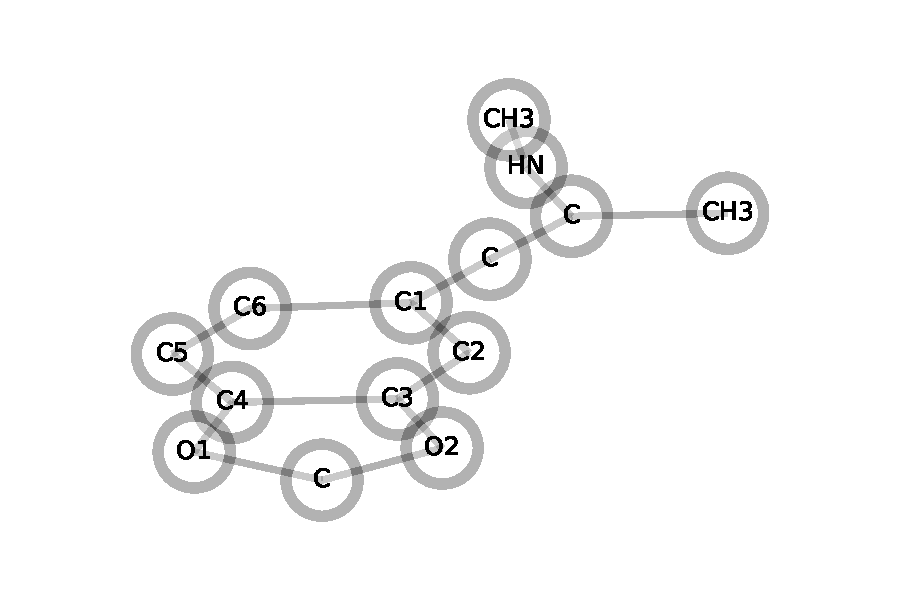
\includegraphics[width=1.0\textwidth]{mdma.pdf}};


\end{scope}

\end{tikzpicture}


\end{document}